\documentclass[../mathNotesPreamble]{subfiles}
\begin{document}
%  \relscale{1.4}
  \section{6.4: Volume by Shells}

  \begin{thmBox*}[Volume by the Shell Method]
    Let $f$ and $g$ be continuous functions with $f(x)\geq g(x)$ on $\sbrkt{a,b}$. If $R$ is the region bounded by the curves $y=f(x)$ and $y=g(x)$ between the lines $x=a$ and $x=b$, the volume of the solid generated when $R$ is revolved about the $y$-axis is
      \[V=\int_a^b \underbrace{2\pi x\vphantom{)}}_{\substack{\textnormal{shell}\\\mathclap{\textnormal{circumference}}}} (\underbrace{f(x)-g(x)}_{\substack{\textnormal{shell}\\\textnormal{height}}})\,dx.\]
  \end{thmBox*}
  \begin{center}
    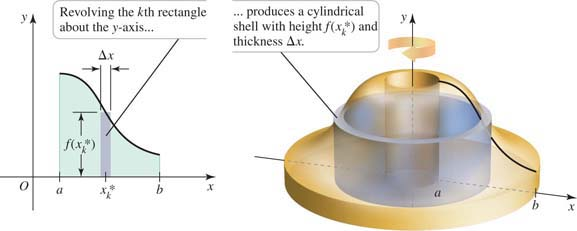
\includegraphics[width=0.6\linewidth]{../images/briggs_06_04/fig06_40}
    \vspace*{\stretch{1}}

    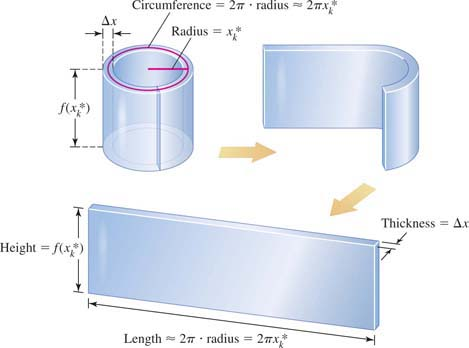
\includegraphics[width=0.5\linewidth]{../images/briggs_06_04/fig06_41}
  \end{center}
  \pagebreak

  \begin{ex*}
    Consider a general region $R$ revolved around the $y$-axis.
  \end{ex*}
  \begin{tasks}[after-item-skip=\stretch{1}, label=](1)
    \task 
      When using the \textbf{disk/washer} method, we integrate with respect to \underline{\hspace*{25mm}}
    \task 
      When using the \textbf{shell} method, we integrate with respect to \underline{\hspace*{25mm}}
  \end{tasks}
  \vspace*{\stretch{1}}
  \begin{ex*}
    Consider a general region $R$ revolved around the $x$-axis.
  \end{ex*}
  \begin{tasks}[after-item-skip=\stretch{1}, label=](1)
    \task 
      When using the \textbf{disk/washer} method, we integrate with respect to \underline{\hspace*{25mm}}
    \task 
      When using the \textbf{shell} method, we integrate with respect to \underline{\hspace*{25mm}}
  \end{tasks}
  \vspace*{\stretch{1}}
  \pagebreak

  \begin{ex*}
    Consider the region bounded between $y=x^3$, $y=8$ and $x=0$.
  \end{ex*}
  \begin{flushright}
    \begin{tikzpicture}
      \begin{axis}[
        grid style={line width=0.3pt, draw=gray!60},
        axis lines=center,
        axis line style={black,->},
        xmin=-2.5, xmax=2.5,
        ymin=-9, ymax=12,
        ymajorticks=false,
        ticklabel style={font=\footnotesize,inner sep=0.5pt,fill=white,opacity=0.5, text opacity=1},
        every axis plot/.append style={line width=0.95pt, color=blue, samples=100},
        width=0.45\linewidth, height=0.3\linewidth
        ]
        \addplot[->, name path=A, ClemsonPurple] expression[domain=-2:2.1]{x^3} node[black, pos=0.8, right, font=\normalsize] {$x^3$};
        \addplot[->, name path=B, ClemsonPurple] [domain=-2.5:2.5] {8} node[black, pos=0.25, above, font=\normalsize] {$y=8$};
        \addplot[fill=HowardsRock!55, opacity=0.75] fill between[of=A and B, soft clip={domain=0:2}];
      \end{axis}
    \end{tikzpicture}
  \end{flushright}
  \begin{tasks}[after-item-skip=\stretch{1}, label=](1)
    \task 
      Use the disk/washer method to setup the integral that represents the volume of the solid generated by rotating the region about the $x$-axis.
    \task 
      about the $y$-axis.
    \task 
      Use the disk/washer method to setup the integral that represents the volume of the solid generated by rotating the region about the line $x=-1$.
    \task 
      about the line $y=8$.
  \end{tasks}
  \vspace*{\stretch{1}}
  \pagebreak

\begin{ex*}
    Consider the region $R$ bounded by $y=4-x^2$, $y=2$, and $x=1$. Use the shell method to setup the integral that represents the volume of the solid generated by rotating the region $R$ about the indicated axis of rotation.
  \end{ex*}
  \newcommand{\parabolicFig}{
    \begin{flushright}
      \vspace*{-\baselineskip}
      \begin{tikzpicture}[scale=0.925]
        \begin{axis}[
          grid style={line width=0.3pt, draw=gray!60},
          axis lines=center,
          axis line style={black,->},
          xmin=-2.7, xmax=2.7,
          ymin=-1, ymax=4.5,
          ymajorticks=false,
          ticklabel style={font=\footnotesize,inner sep=0.5pt,fill=white,opacity=0.5, text opacity=1},
          every axis plot/.append style={line width=0.95pt, color=blue, samples=100},
          width=0.45\linewidth, height=0.3\linewidth
          ]
          \addplot[->, name path=A, ClemsonPurple] expression[domain=-2.5:2.5]{4-x^2} node[black, pos=0.71, right, font=\normalsize, xshift=-2pt] {$4-x^2$};
          \addplot[-, name path=B, ClemsonOrange] [domain=-2.5:2.5] {2} node[black, pos=0.4, above, font=\normalsize] {$y=2$};
          \addplot[fill=HowardsRock!55, opacity=0.75] fill between[of=A and B, soft clip={domain=1:1.414}];
          \draw[ClemsonOrange] (axis cs: 1,-2)--(axis cs: 1,5);
        \end{axis}
      \end{tikzpicture}
    \end{flushright}
    }
  
  \begin{tasks}[after-item-skip=\stretch{1}, label=](1)
    \task 
      about $x$-axis,
      \parabolicFig
    \task 
      about $y$-axis,
      \parabolicFig
    \task 
      about the line $x=-2$,
      \parabolicFig
    \task 
      about the line $y=2$.
      \parabolicFig
  \end{tasks}
  \pagebreak

  \begin{ex*}
    Consider the region bounded by $y=\dfrac{1}{x+1}$ and $y=1-\dfrac{x}{3}$. Use both the disk/washer method and shell method to find the volume of the solid generated when $R$ is rotated about the $x$-axis.
  \end{ex*}
  \vspace*{\stretch{1}}
  \pagebreak

  \begin{ex*}
    Determine if the following statements are true.
  \end{ex*}
  \begin{tasks}[after-item-skip=\stretch{1}, label=](1)
    \task 
      When using the shell method, the axis of the cylindrical shells is parallel to the axis of revolution.
    \task 
      If a region is revolved about the $y$-axis, then the shell method must be used.
    \task 
      If a region is revolved about the $x$-axis, it is possible to use the disk/washer method and integrate with respect to $x$.
  \end{tasks}
  \vspace*{\stretch{1}}
  \pagebreak

\end{document}
